\documentclass{standalone}
\usepackage{graphicx}	
\usepackage{amssymb, amsmath}
\usepackage{color}

\usepackage{tikz}
\usetikzlibrary{intersections, backgrounds}

\definecolor{light}{RGB}{220, 188, 188}
\definecolor{mid}{RGB}{185, 124, 124}
\definecolor{dark}{RGB}{143, 39, 39}
\definecolor{highlight}{RGB}{180, 31, 180}
\definecolor{gray10}{gray}{0.1}
\definecolor{gray20}{gray}{0.2}
\definecolor{gray30}{gray}{0.3}
\definecolor{gray40}{gray}{0.4}
\definecolor{gray60}{gray}{0.6}
\definecolor{gray70}{gray}{0.7}
\definecolor{gray80}{gray}{0.8}
\definecolor{gray90}{gray}{0.9}
\definecolor{gray95}{gray}{0.95}

\newcommand*{\offset}{0.025}

\begin{document}

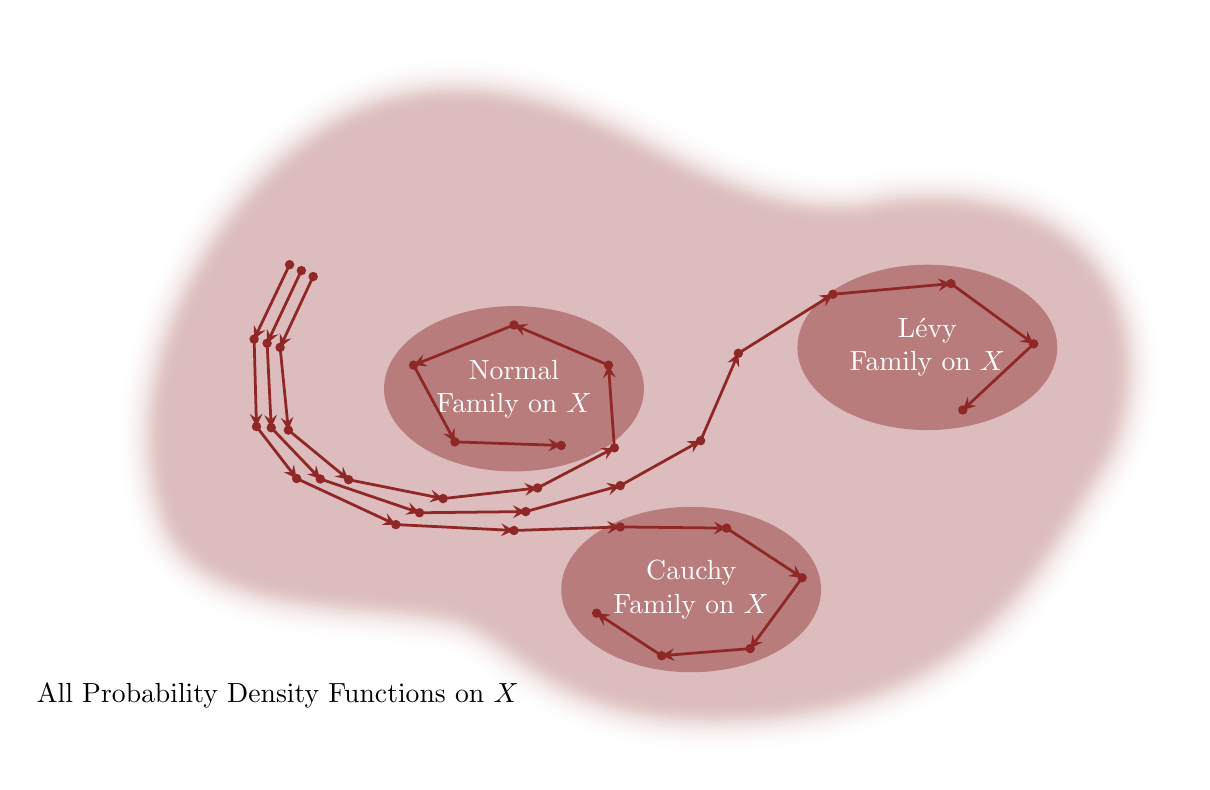
\begin{tikzpicture}[scale=0.3, thick]               
 \pgfmathsetmacro{\dx}{18}
 
 \foreach \i in {0.025, 0.05, ..., 1} {
   \draw[line width={40 * \i}, opacity={exp(-5 * \i))}, light] 
     (-20, -2)
    .. controls (-22, 4) and (-17, 12) .. (-12, 14)  
    .. controls (-7, 16) and (-2, 13) .. (0, 12)
    .. controls (2, 11) and (6, 9) .. (10, 10)
    .. controls (20, 11) and (20, 3) .. (18, 0)
    .. controls (15.5, -4) and (13, -9.5) .. (4, -10)
    .. controls (-4, -10.5) and (-5, -7) .. (-8, -6)
    .. controls (-11, -5) and (-19, -6) .. (-20, -2);
  }
  
  \fill [fill=light] (-20, -2)
    .. controls (-22, 4) and (-17, 12) .. (-12, 14)  
    .. controls (-7, 16) and (-2, 13) .. (0, 12)
    .. controls (2, 11) and (6, 9) .. (10, 10)
    .. controls (20, 11) and (20, 3) .. (18, 0)
    .. controls (15.5, -4) and (13, -9.5) .. (4, -10)
    .. controls (-4, -10.5) and (-5, -7) .. (-8, -6)
    .. controls (-11, -5) and (-19, -6) .. (-20, -2);
    
  \node [] at (-16, -10) { All Probability Density Functions on $X$ };
    
  \fill[mid] (-6, 3) circle [x radius=5.5, y radius=3.5]
  node [color=white, align=center] {Normal\\Family on $X$};

  \fill[mid] (1.5, -5.5) circle [x radius=5.5, y radius=3.5]
  node [color=white, align=center] {Cauchy\\Family on $X$};
  
  \fill[mid] (11.5, 4.75) circle [x radius=5.5, y radius=3.5]
  node [color=white, align=center] {L\'{e}vy\\Family on $X$};
  
  %\draw [color=dark] (-14.5, 7.75) 
  %  .. controls (-16, 5) and (-17.5, 2.75) .. (-14.5, 0)
  %  .. controls (-11.5, -2.75) and (-5, -1.5) .. (-3, -0.5)
  %  .. controls (-1, 0.5) and (-0.5, 3) .. (-2.5, 4.5)
  %  .. controls (-4.5, 6) and (-7, 6) .. (-9, 5)
  %  .. controls (-11, 4) and (-11, 2) .. (-9, 1)
  %  .. controls (-7, 0) and (-5, 0) .. (-3, 1);
  
  %\node [color=dark] at (-13.5, 7.75) { $\pi_{1}$ };
  \fill[dark] (-14.5, 7.75) circle (0.2);
  
  \draw[->, >=stealth, line width=1, color=dark] (-14.5, 7.75) -- (-15.9, 4.75);
  
  \fill[dark] (-15.9, 4.75) circle (0.2);
  
  \draw[->, >=stealth, line width=1, color=dark] (-15.9, 4.75) -- (-15.55, 1.25);
  
  \fill[dark] (-15.55, 1.25) circle (0.2);
  
  \draw[->, >=stealth, line width=1, color=dark] (-15.55, 1.25) -- (-13, -0.85);
  
  \fill[dark] (-13, -0.85) circle (0.2);
  
  \draw[->, >=stealth, line width=1, color=dark] (-13, -0.85) -- (-9, -1.65);
  
  \fill[dark] (-9, -1.65) circle (0.2);
  
  \draw[->, >=stealth, line width=1, color=dark] (-9, -1.65) -- (-5, -1.2);
  
  \fill[dark] (-5, -1.2) circle (0.2);
  
  \draw[->, >=stealth, line width=1, color=dark] (-5, -1.2) -- (-1.75, 0.5);
  
  \fill[dark] (-1.75, 0.5) circle (0.2);
  
  \draw[->, >=stealth, line width=1, color=dark] (-1.75, 0.5) -- (-2, 4);
  
  \fill[dark] (-2, 4) circle (0.2);
  
  \draw[->, >=stealth, line width=1, color=dark] (-2, 4) -- (-6, 5.7);
  
  \fill[dark] (-6, 5.7) circle (0.2);
  
  \draw[->, >=stealth, line width=1, color=dark] (-6, 5.7) -- (-10.25, 4);
  
  \fill[dark] (-10.25, 4) circle (0.2);
  
  \draw[->, >=stealth, line width=1, color=dark] (-10.25, 4) -- (-8.5, 0.75);
  
  \fill[dark] (-8.5, 0.75) circle (0.2);
  
  \draw[->, >=stealth, line width=1, color=dark] (-8.5, 0.75) -- (-4, 0.6);
  
  \fill[dark] (-4, 0.6) circle (0.2);
  
  %\draw [color=dark] (-15, 8) 
  %  .. controls (-16.5, 5.25) and (-18, 2.5) .. (-15, -0.25)
  %  .. controls (-12, -3) and (-5, -2.75) .. (-3, -1.75)
  %  .. controls (-1, -0.75) and (2.5, 0) .. (3, 3)
  %  .. controls (3.5, 6.5) and (8.5, 7.5) .. (11.5, 7.5)
  %  .. controls (13.5, 7.5) and (16, 6.75) .. (16, 4.75)
  %  .. controls (16, 2.75) and (13.5, 2) .. (11.5, 2);
 
  %\node [color=dark] at (-14.5, 8.75) { $\pi_{2}$ };
  \fill[dark] (-15, 8) circle (0.2);
  
  \draw[->, >=stealth, line width=1, color=dark] (-15, 8) -- (-16.45, 4.925);
  
  \fill[dark] (-16.45, 4.925) circle (0.2);
  
  \draw[->, >=stealth, line width=1, color=dark] (-16.45, 4.925) -- (-16.275, 1.35);
  
  \fill[dark] (-16.275, 1.35) circle (0.2);
  
  \draw[->, >=stealth, line width=1, color=dark] (-16.275, 1.35) -- (-14.2, -0.82);
  
  \fill[dark] (-14.2, -0.82) circle (0.2);
  
  \draw[->, >=stealth, line width=1, color=dark] (-14.2, -0.82) -- (-10, -2.25);
  
  \fill[dark] (-10, -2.25) circle (0.2);
  
  \draw[->, >=stealth, line width=1, color=dark] (-10, -2.25) -- (-5.5, -2.2);
  
  \fill[dark] (-5.5, -2.2) circle (0.2);
  
  \draw[->, >=stealth, line width=1, color=dark] (-5.5, -2.2) -- (-1.5, -1.1);
  
  \fill[dark] (-1.5, -1.1) circle (0.2);
  
  \draw[->, >=stealth, line width=1, color=dark] (-1.5, -1.1) -- (1.9, 0.8);
  
  \fill[dark] (1.9, 0.8) circle (0.2);
  
  \draw[->, >=stealth, line width=1, color=dark] (1.9, 0.8) -- (3.5, 4.5);
  
  \fill[dark] (3.5, 4.5) circle (0.2);
  
  \draw[->, >=stealth, line width=1, color=dark] (3.5, 4.5) -- (7.5, 7);
  
  \fill[dark] (7.5, 7) circle (0.2);
  
  \draw[->, >=stealth, line width=1, color=dark] (7.5, 7) -- (12.5, 7.45);
  
  \fill[dark] (12.5, 7.45) circle (0.2);
  
  \draw[->, >=stealth, line width=1, color=dark] (12.5, 7.45) -- (16, 4.9);
  
  \fill[dark] (16, 4.9) circle (0.2);
  
  \draw[->, >=stealth, line width=1, color=dark] (16, 4.9) -- (13, 2.1);
  
  \fill[dark] (13, 2.1) circle (0.2);
  
  %\draw [color=dark] (-15.5, 8.25) 
  %  .. controls (-17, 5.5) and (-18.5, 2.25) .. (-15.5, -0.5)
  %  .. controls (-12, -4.25) and (-5, -2.75) .. (1.5, -2.75)
  %  .. controls (3.5, -2.75) and (6.25, -3.5) .. (6.25, -5.5)
  %  .. controls (6.25, -7.5) and (3.5, -8.5) .. (1.5, -8.5)
  %  .. controls (-0.5, -8.5) and (-2.5, -7.5) .. (-2.5, -6.5);
    
  %\node [color=dark] at (-16, 9.25) { $\pi_{3}$ };
  \fill[dark] (-15.5, 8.25) circle (0.2);
  
  \draw[->, >=stealth, line width=1, color=dark] (-15.5, 8.25) -- (-17, 5.1);
  
  \fill[dark] (-17, 5.1) circle (0.2);
  
  \draw[->, >=stealth, line width=1, color=dark] (-17, 5.1) -- (-16.9, 1.4);
  
  \fill[dark] (-16.9, 1.4) circle (0.2);
  
  \draw[->, >=stealth, line width=1, color=dark] (-16.9, 1.4) -- (-15.2, -0.8);
  
  \fill[dark] (-15.2, -0.8) circle (0.2);
  
  \draw[->, >=stealth, line width=1, color=dark] (-15.2, -0.8) -- (-11, -2.75);
  
  \fill[dark] (-11, -2.75) circle (0.2);
  
  \draw[->, >=stealth, line width=1, color=dark] (-11, -2.75) -- (-6, -3);
  
  \fill[dark] (-6, -3) circle (0.2);
  
  \draw[->, >=stealth, line width=1, color=dark] (-6, -3) -- (-1.5, -2.85);
  
  \fill[dark] (-1.5, -2.85) circle (0.2);
  
  \draw[->, >=stealth, line width=1, color=dark] (-1.5, -2.85) -- (3, -2.9);
  
  \fill[dark] (3, -2.9) circle (0.2);
  
  \draw[->, >=stealth, line width=1, color=dark] (3, -2.9) -- (6.2, -5);
  
  \fill[dark] (6.2, -5) circle (0.2);
  
  \draw[->, >=stealth, line width=1, color=dark] (6.2, -5) -- (4, -8);
  
  \fill[dark] (4, -8) circle (0.2);
  
  \draw[->, >=stealth, line width=1, color=dark] (4, -8) -- (0.25, -8.3);
  
  \fill[dark] (0.25, -8.3) circle (0.2);
  
  \draw[->, >=stealth, line width=1, color=dark] (0.25, -8.3) -- (-2.5, -6.5);
  
  \fill[dark] (-2.5, -6.5) circle (0.2);

\end{tikzpicture}

\end{document}   